\documentclass{standalone}
\usepackage{tikz}
\usetikzlibrary{patterns, positioning}


\begin{document}
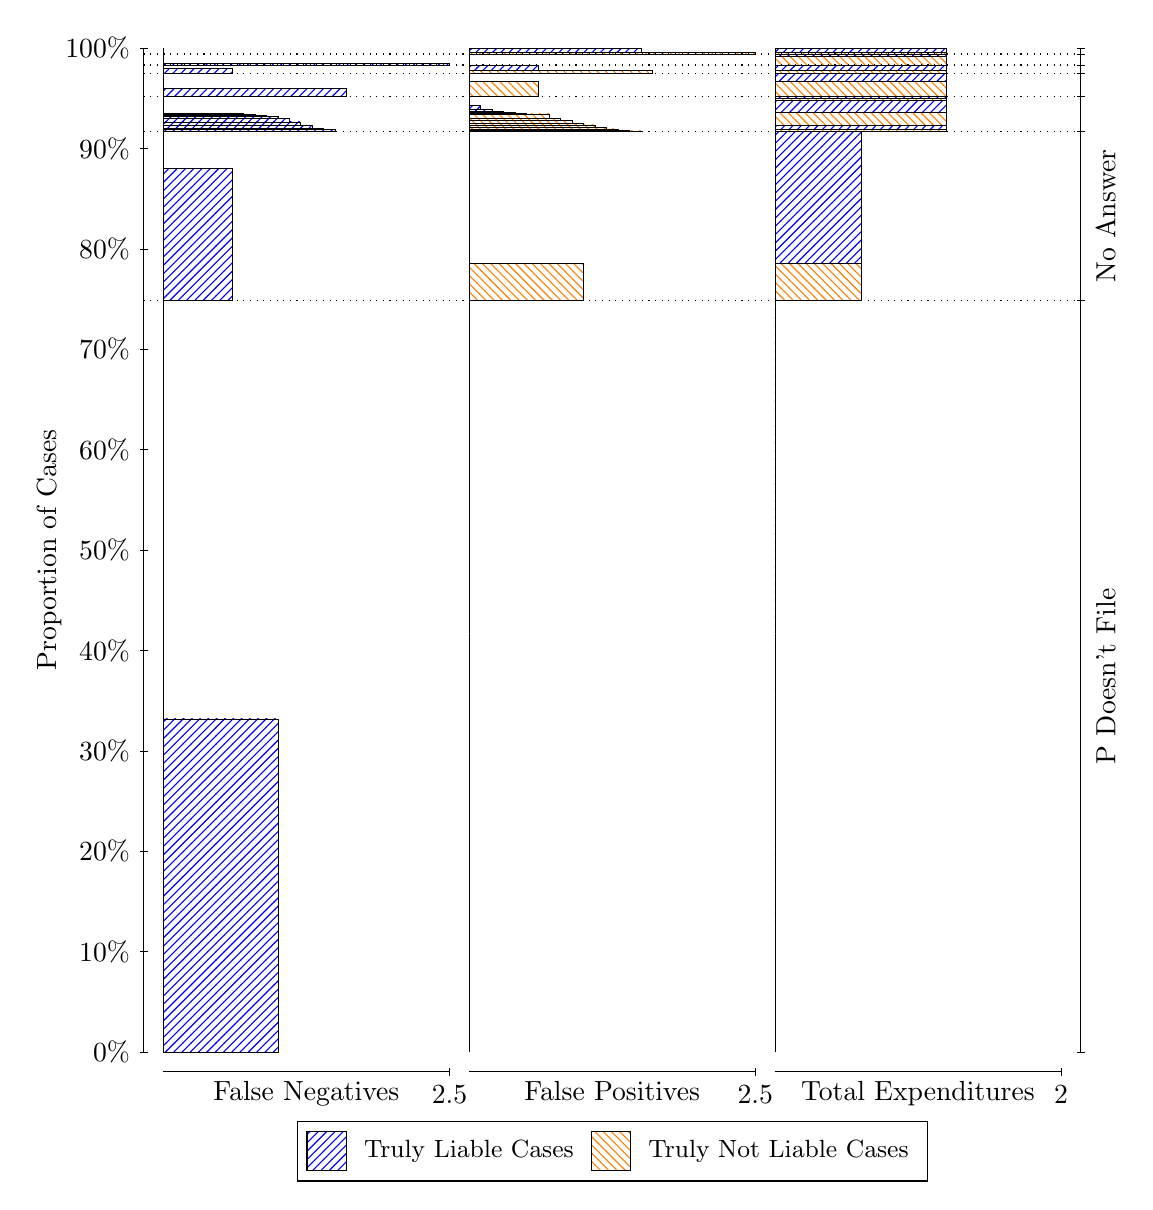
\begin{tikzpicture}
\draw[black, very thin] (1.5,1.75) -- (1.5,14.5);
\node[rotate=90, text=black, anchor=center] at (0.3, 8.125) {Proportion of Cases};
\draw[black, very thin] (1.45,1.75) -- (1.55,1.75);
\node[text=black, anchor=east] at (1.45, 1.75) {0\%};
\draw[black, very thin] (1.45,3.025) -- (1.55,3.025);
\node[text=black, anchor=east] at (1.45, 3.025) {10\%};
\draw[black, very thin] (1.45,4.3) -- (1.55,4.3);
\node[text=black, anchor=east] at (1.45, 4.3) {20\%};
\draw[black, very thin] (1.45,5.575) -- (1.55,5.575);
\node[text=black, anchor=east] at (1.45, 5.575) {30\%};
\draw[black, very thin] (1.45,6.85) -- (1.55,6.85);
\node[text=black, anchor=east] at (1.45, 6.85) {40\%};
\draw[black, very thin] (1.45,8.125) -- (1.55,8.125);
\node[text=black, anchor=east] at (1.45, 8.125) {50\%};
\draw[black, very thin] (1.45,9.4) -- (1.55,9.4);
\node[text=black, anchor=east] at (1.45, 9.4) {60\%};
\draw[black, very thin] (1.45,10.675) -- (1.55,10.675);
\node[text=black, anchor=east] at (1.45, 10.675) {70\%};
\draw[black, very thin] (1.45,11.95) -- (1.55,11.95);
\node[text=black, anchor=east] at (1.45, 11.95) {80\%};
\draw[black, very thin] (1.45,13.225) -- (1.55,13.225);
\node[text=black, anchor=east] at (1.45, 13.225) {90\%};
\draw[black, very thin] (1.45,14.5) -- (1.55,14.5);
\node[text=black, anchor=east] at (1.45, 14.5) {100\%};

\draw[black, very thin] (13.4,1.75) -- (13.4,14.5);
\draw[black, very thin] (13.35,1.75) -- (13.45,1.75);
\node[anchor=west] at (13.35, 1.75) {};
\draw[black, very thin] (13.35,11.293) -- (13.45,11.293);
\node[anchor=west] at (13.35, 11.293) {};
\draw[black, very thin] (13.35,13.441) -- (13.45,13.441);
\node[anchor=west] at (13.35, 13.441) {};
\draw[black, very thin] (13.35,13.889) -- (13.45,13.889);
\node[anchor=west] at (13.35, 13.889) {};
\draw[black, very thin] (13.35,14.175) -- (13.45,14.175);
\node[anchor=west] at (13.35, 14.175) {};
\draw[black, very thin] (13.35,14.284) -- (13.45,14.284);
\node[anchor=west] at (13.35, 14.284) {};
\draw[black, very thin] (13.35,14.424) -- (13.45,14.424);
\node[anchor=west] at (13.35, 14.424) {};
\draw[black, very thin] (13.35,14.5) -- (13.45,14.5);
\node[anchor=west] at (13.35, 14.5) {};

\draw[black, very thin, pattern color=blue, pattern=north east lines] (1.75,1.75) rectangle (3.2033,5.98);
\draw[black, very thin, pattern color=orange, pattern=north west lines] (1.75,5.98) rectangle (1.75,11.293);
\draw[black, very thin, pattern color=blue, pattern=north east lines] (1.75,11.293) rectangle (2.622,12.968);
\draw[black, very thin, pattern color=orange, pattern=north west lines] (1.75,12.968) rectangle (1.75,13.441);
\draw[black, very thin, pattern color=blue, pattern=north east lines] (1.75,13.441) rectangle (3.93,13.469);
\draw[black, very thin, pattern color=blue, pattern=north east lines] (1.75,13.469) rectangle (3.7847,13.479);
\draw[black, very thin, pattern color=blue, pattern=north east lines] (1.75,13.479) rectangle (3.6393,13.518);
\draw[black, very thin, pattern color=blue, pattern=north east lines] (1.75,13.518) rectangle (3.494,13.562);
\draw[black, very thin, pattern color=blue, pattern=north east lines] (1.75,13.562) rectangle (3.3487,13.607);
\draw[black, very thin, pattern color=blue, pattern=north east lines] (1.75,13.607) rectangle (3.2033,13.631);
\draw[black, very thin, pattern color=blue, pattern=north east lines] (1.75,13.631) rectangle (3.058,13.648);
\draw[black, very thin, pattern color=blue, pattern=north east lines] (1.75,13.648) rectangle (2.9127,13.656);
\draw[black, very thin, pattern color=blue, pattern=north east lines] (1.75,13.656) rectangle (2.7673,13.666);
\draw[black, very thin, pattern color=orange, pattern=north west lines] (1.75,13.666) rectangle (1.75,13.889);
\draw[black, very thin, pattern color=blue, pattern=north east lines] (1.75,13.889) rectangle (4.0753,13.992);
\draw[black, very thin, pattern color=orange, pattern=north west lines] (1.75,13.992) rectangle (1.75,14.175);
\draw[black, very thin, pattern color=blue, pattern=north east lines] (1.75,14.175) rectangle (2.622,14.241);
\draw[black, very thin, pattern color=orange, pattern=north west lines] (1.75,14.241) rectangle (1.75,14.284);
\draw[black, very thin, pattern color=blue, pattern=north east lines] (1.75,14.284) rectangle (5.3833,14.309);
\draw[black, very thin, pattern color=orange, pattern=north west lines] (1.75,14.309) rectangle (1.75,14.424);
\draw[black, very thin, pattern color=orange, pattern=north west lines] (1.75,14.424) rectangle (1.75,14.448);
\draw[black, very thin, pattern color=blue, pattern=north east lines] (1.75,14.448) rectangle (1.75,14.5);
\draw[black, very thin, pattern color=orange, pattern=north west lines] (5.6333,1.75) rectangle (5.6333,7.0633);
\draw[black, very thin, pattern color=blue, pattern=north east lines] (5.6333,7.0633) rectangle (5.6333,11.293);
\draw[black, very thin, pattern color=orange, pattern=north west lines] (5.6333,11.293) rectangle (7.0867,11.766);
\draw[black, very thin, pattern color=blue, pattern=north east lines] (5.6333,11.766) rectangle (5.6333,13.441);
\draw[black, very thin, pattern color=orange, pattern=north west lines] (5.6333,13.441) rectangle (7.8133,13.449);
\draw[black, very thin, pattern color=orange, pattern=north west lines] (5.6333,13.449) rectangle (7.668,13.457);
\draw[black, very thin, pattern color=orange, pattern=north west lines] (5.6333,13.457) rectangle (7.5227,13.474);
\draw[black, very thin, pattern color=orange, pattern=north west lines] (5.6333,13.474) rectangle (7.3773,13.494);
\draw[black, very thin, pattern color=orange, pattern=north west lines] (5.6333,13.494) rectangle (7.232,13.524);
\draw[black, very thin, pattern color=orange, pattern=north west lines] (5.6333,13.524) rectangle (7.0867,13.545);
\draw[black, very thin, pattern color=orange, pattern=north west lines] (5.6333,13.545) rectangle (6.9413,13.583);
\draw[black, very thin, pattern color=orange, pattern=north west lines] (5.6333,13.583) rectangle (6.796,13.603);
\draw[black, very thin, pattern color=orange, pattern=north west lines] (5.6333,13.603) rectangle (6.6507,13.664);
\draw[black, very thin, pattern color=blue, pattern=north east lines] (5.6333,13.664) rectangle (6.36,13.674);
\draw[black, very thin, pattern color=blue, pattern=north east lines] (5.6333,13.674) rectangle (6.2147,13.682);
\draw[black, very thin, pattern color=blue, pattern=north east lines] (5.6333,13.682) rectangle (6.0693,13.699);
\draw[black, very thin, pattern color=blue, pattern=north east lines] (5.6333,13.699) rectangle (5.924,13.722);
\draw[black, very thin, pattern color=blue, pattern=north east lines] (5.6333,13.722) rectangle (5.7787,13.768);
\draw[black, very thin, pattern color=blue, pattern=north east lines] (5.6333,13.768) rectangle (5.6333,13.889);
\draw[black, very thin, pattern color=orange, pattern=north west lines] (5.6333,13.889) rectangle (6.5053,14.072);
\draw[black, very thin, pattern color=blue, pattern=north east lines] (5.6333,14.072) rectangle (5.6333,14.175);
\draw[black, very thin, pattern color=orange, pattern=north west lines] (5.6333,14.175) rectangle (7.9587,14.218);
\draw[black, very thin, pattern color=blue, pattern=north east lines] (5.6333,14.218) rectangle (6.5053,14.284);
\draw[black, very thin, pattern color=orange, pattern=north west lines] (5.6333,14.284) rectangle (5.6333,14.399);
\draw[black, very thin, pattern color=blue, pattern=north east lines] (5.6333,14.399) rectangle (5.6333,14.424);
\draw[black, very thin, pattern color=orange, pattern=north west lines] (5.6333,14.424) rectangle (9.2667,14.448);
\draw[black, very thin, pattern color=blue, pattern=north east lines] (5.6333,14.448) rectangle (7.8133,14.5);
\draw[black, very thin, pattern color=orange, pattern=north west lines] (9.5167,1.75) rectangle (9.5167,7.0633);
\draw[black, very thin, pattern color=blue, pattern=north east lines] (9.5167,7.0633) rectangle (9.5167,11.293);
\draw[black, very thin, pattern color=orange, pattern=north west lines] (9.5167,11.293) rectangle (10.607,11.766);
\draw[black, very thin, pattern color=blue, pattern=north east lines] (9.5167,11.766) rectangle (10.607,13.441);
\draw[black, very thin, pattern color=orange, pattern=north west lines] (9.5167,13.441) rectangle (11.697,13.471);
\draw[black, very thin, pattern color=blue, pattern=north east lines] (9.5167,13.471) rectangle (11.697,13.516);
\draw[black, very thin, pattern color=orange, pattern=north west lines] (9.5167,13.516) rectangle (11.697,13.685);
\draw[black, very thin, pattern color=blue, pattern=north east lines] (9.5167,13.685) rectangle (11.697,13.839);
\draw[black, very thin, pattern color=orange, pattern=north west lines] (9.5167,13.839) rectangle (11.697,13.863);
\draw[black, very thin, pattern color=blue, pattern=north east lines] (9.5167,13.863) rectangle (11.697,13.889);
\draw[black, very thin, pattern color=orange, pattern=north west lines] (9.5167,13.889) rectangle (11.697,14.072);
\draw[black, very thin, pattern color=blue, pattern=north east lines] (9.5167,14.072) rectangle (11.697,14.175);
\draw[black, very thin, pattern color=orange, pattern=north west lines] (9.5167,14.175) rectangle (11.697,14.218);
\draw[black, very thin, pattern color=blue, pattern=north east lines] (9.5167,14.218) rectangle (11.697,14.284);
\draw[black, very thin, pattern color=orange, pattern=north west lines] (9.5167,14.284) rectangle (11.697,14.399);
\draw[black, very thin, pattern color=blue, pattern=north east lines] (9.5167,14.399) rectangle (11.697,14.424);
\draw[black, very thin, pattern color=orange, pattern=north west lines] (9.5167,14.424) rectangle (11.697,14.448);
\draw[black, very thin, pattern color=blue, pattern=north east lines] (9.5167,14.448) rectangle (11.697,14.5);
\draw[black, dotted] (1.5,11.293) -- (13.4,11.293);
\draw[black, dotted] (1.5,13.441) -- (13.4,13.441);
\draw[black, dotted] (1.5,13.889) -- (13.4,13.889);
\draw[black, dotted] (1.5,14.175) -- (13.4,14.175);
\draw[black, dotted] (1.5,14.284) -- (13.4,14.284);
\draw[black, dotted] (1.5,14.424) -- (13.4,14.424);
\draw[black, very thin] (1.75,1.5) -- (5.3833,1.5);
\node[text=black, anchor=north] at (3.5667, 1.5) {False Negatives};
\draw[black, very thin] (5.3833,1.45) -- (5.3833,1.55);
\node[text=black, anchor=north] at (5.3833, 1.45) {2.5};

\draw[black, very thin] (5.6333,1.5) -- (9.2667,1.5);
\node[text=black, anchor=north] at (7.45, 1.5) {False Positives};
\draw[black, very thin] (9.2667,1.45) -- (9.2667,1.55);
\node[text=black, anchor=north] at (9.2667, 1.45) {2.5};

\draw[black, very thin] (9.5167,1.5) -- (13.15,1.5);
\node[text=black, anchor=north] at (11.333, 1.5) {Total Expenditures};
\draw[black, very thin] (13.15,1.45) -- (13.15,1.55);
\node[text=black, anchor=north] at (13.15, 1.45) {2};

\node[text=black, centered, rotate=90] at (13.72, 6.5216) {P Doesn't File};
\node[text=black, centered, rotate=90] at (13.72, 12.367) {No Answer};






\draw (7.449999999999999,1.5) node[draw=none] (baseCoordinate) {};
\begin{scope}[align=center]
        \matrix[scale=0.5, draw=black, below=0.5cm of baseCoordinate, nodes={draw}, column sep=0.1cm]{
            \node[rectangle, draw, minimum width=0.5cm, minimum height=0.5cm, pattern color=blue, pattern=north east lines] {}; &
            \node[draw=none, font=\small, text=black] (B) {Truly Liable Cases}; &
            \node[rectangle, draw, minimum width=0.5cm, minimum height=0.5cm, pattern color=orange, pattern=north west lines] {}; &
            \node[draw=none, font=\small, text=black] (B) {Truly Not Liable Cases}; \\
            };
\end{scope}

\end{tikzpicture}
\end{document}